%"The PDF file may contain up to 25 pages of reference material, single-sided, letter or A4 size, with text and illustrations readable by a person with correctable eyesight without magnification from a distance of 1/2 meter."        
\documentclass[10pt,landscape,twocolumn,a4paper,notitlepage]{article}
\usepackage[utf8]{inputenc} % Solo si usas pdfLaTeX
\usepackage[T1]{fontenc}
\usepackage[english,activeacute]{babel}
\usepackage{hyperref}
\usepackage{fancyhdr}
\usepackage{lastpage}
\usepackage{listings}
\usepackage{amssymb}
\usepackage[usenames,dvipsnames]{color}
\usepackage{graphicx}
\usepackage{wrapfig}
\usepackage{amsmath}
\usepackage{makeidx}

\input{preamble.tex}
\newcommand{\mytitle}{UTO-FNI  - La maquinita y sus subordinados}
\pagestyle{fancy}
\fancyhf{}
\fancyhead[LO]{\textbf{\mytitle}}
\fancyhead[C]{\leftmark\ -\ \rightmark}
\fancyhead[RO]{Page \thepage\ of \pageref{LastPage}}
\renewcommand{\headrulewidth}{0.4pt}

\begin{document}

% Gracias Demetrio
\begin{center}
    {\LARGE\textbf{La Union hace la Fuerza}} \\[0.5cm]
    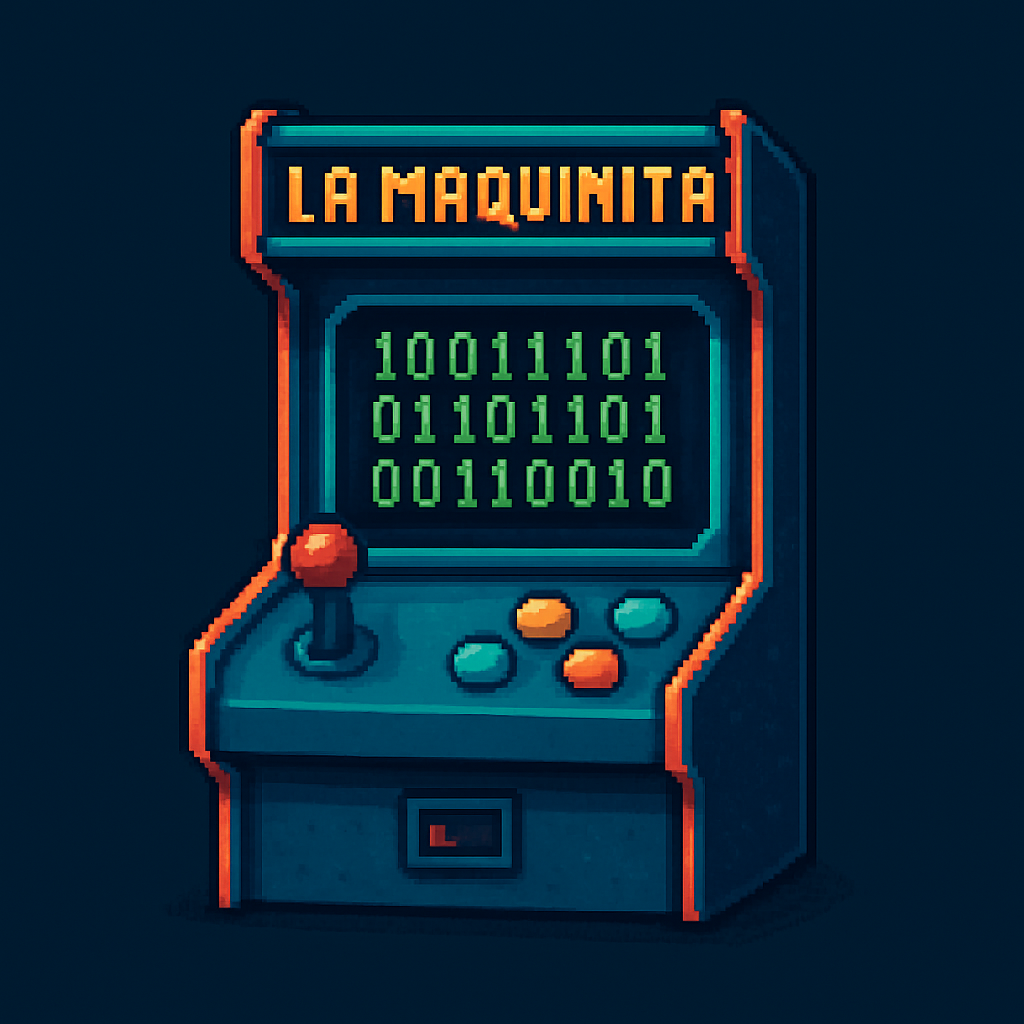
\includegraphics[width=5.5cm]{img/maquinita_dark.png}
\end{center}
\tableofcontents\newpage
\section{Data Structures}
\subsection{Priority Queue de minimos}
\cppfile{data_structures/pq_minimos.cpp}
\subsection{Priority Queue de maximos}
\cppfile{data_structures/pq_max.cpp}
\subsection{Tabla Aditiva - Partial Sum o Prefix Sum}
\cppfile{varios/prefix_sum.cpp}

% Operaciones con bits en C++
\section{Operaciones con bits en C++}
\subsection{Tabla bitwise}
 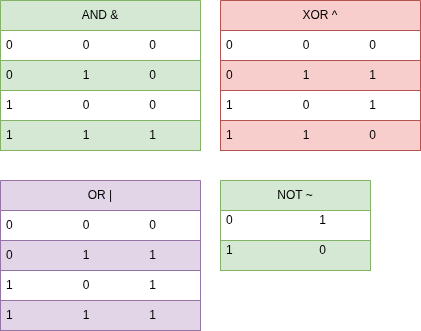
\includegraphics[width=0.5\textwidth]{img/tablabits.png}
\subsection{Funciones utilices de C++}
\subsubsection{popcount}
Para obtener el numero de bits encendidos en un entero
\cppfile{vitsitos/pop_count.cpp}
Version para numeros de 64bits (long long)
\cppfile{vitsitos/pop_count_ll.cpp}
Hack bits
\cppfile{vitsitos/hack.cpp}
\subsection{Gcd Bits}
\cppfile{vitsitos/gcdbits.cpp}

\section{Grafos}
\subsection{Revision 8 adyacentes}
\cppfile{graphs/8adyacence.cpp}
\subsection{Algoritmo Dijkstra}
\cppfile{graphs/dijkstra.cpp}
\subsection{Algoritmo Bellman-Ford}
\cppfile{graphs/bellmanford.cpp}
\subsection{Conteo de componentes conexas}
\cppfile{graphs/conexas.cpp}
\subsection{Union Find}
\cppfile{graphs/unionfind.cpp}
\subsection{Graph Diameter}
\cppfile{graphs/diameterfunction.cpp}


\section{Manejo de Strings}
\subsection{Sub String}
\cppfile{string/substring.cpp}
\subsection{KMP}
\cppfile{string/kmp.cpp}
\section{Trucos Varios}
\subsection{Next Permutation}
\cppfile{varios/next_permutation.cpp}
\subsection{Uso de Fixed}
\cppfile{varios/fixed.cpp}
\subsection{Equivante fixed con printf}
\cppfile{varios/equivante.cpp}
\subsection{iota}
Para generar arreglos consecutivos
\cppfile{varios/iota.cpp}
\subsection{Conversion de unidades}
\cppfile{varios/conversiones.cpp}
\subsection{Salidas varias}
\cppfile{varios/salidas.cpp}
\subsection{Aritmetica con Strings}
\cppfile{varios/arithstring.cpp}
\subsection{Aritmetica con Strings segun deepseek}
\cppfile{varios/deepseek.cpp}
\subsection{Problema M codigo}
\cppfile{varios/codigom.cpp}
\subsection{Matriz Viborita}
\cppfile{varios/viborita.cpp}
\subsection{Triangulo de Pascal}
\cppfile{varios/pascal.cpp}

\section{Geometry}
\subsection{Basicas}
\begin{align}
  &\textbf{Distancia entre dos puntos:} \quad d(P,Q)=\sqrt{(x_2-x_1)^2+(y_2-y_1)^2} \\
  &\textbf{Producto punto:} \quad \mathbf{a}\cdot\mathbf{b}=a_x b_x + a_y b_y \\
  &\textbf{Producto cruz (2D):} \quad \mathbf{a}\times\mathbf{b}=a_x b_y - a_y b_x \\
  &\textbf{Norma de vector:} \quad \|\mathbf{a}\|=\sqrt{a_x^2+a_y^2}
\end{align}

\subsection{Triángulos}
\begin{align}
  &\textbf{Área (1/2 base\,$\times$\,altura):} \quad A=\tfrac12|\mathbf{AB}\times\mathbf{AC}| \\
  &\textbf{Herón:} \quad s=\tfrac{a+b+c}{2}, \quad A=\sqrt{s(s-a)(s-b)(s-c)} \\
  &\textbf{Circunradio:} \quad R=\frac{abc}{4A}, \quad \text{Inradio: } r=\frac{2A}{a+b+c} \\
  &\textbf{Incentro:} \quad I=\frac{aA + bB + cC}{a+b+c}
\end{align}

\subsection{Polígonos}
\begin{align}
  &\textbf{Área (shoelace):} \quad A=\tfrac12\Bigl|\sum_{i=0}^{n-1}(x_i y_{i+1} - x_{i+1} y_i)\Bigr| \\
  &\textbf{Centroide:} \\
  &\quad C_x=\frac{1}{6A}\sum_{i}(x_i+x_{i+1})(x_i y_{i+1}-x_{i+1}y_i), \\ 
  &\quad C_y=\frac{1}{6A}\sum_{i}(y_i+y_{i+1})(x_i y_{i+1}-x_{i+1}y_i)
\end{align}

\subsection{Círculos}
\begin{align}
  &\textbf{Ecuación:} \quad (x-h)^2+(y-k)^2=r^2 \\
  &\textbf{Intersección círculo-círculo:} \\
  &\quad d=\|O_1O_2\|, \quad a=\frac{R^2 - r^2 + d^2}{2d}, \quad h=\sqrt{R^2-a^2} \\
  &\quad \text{Puntos }P_1, P_2 = P_0 \pm h\frac{(O_2-O_1)^{\perp}}{d} \\
  &\textbf{Área intersección:} \\
  &\quad A=R^2\cos^{-1}\Bigl(\frac{d^2+R^2-r^2}{2dR}\Bigr)
        +r^2\cos^{-1}\Bigl(\frac{d^2+r^2-R^2}{2dr}\Bigr)\\
  &\quad\; -\tfrac12\sqrt{(-d+R+r)(d+R-r)(d-R+r)(d+R+r)}
\end{align}

\subsection{Vectores y Operaciones}
\begin{align}
  &\textbf{Conversión polar→cartesiano:} \quad x=r\cos\theta,\;y=r\sin\theta \\
  &\textbf{Conversión cartesiano→polar:} \quad r=\sqrt{x^2+y^2},\;\theta=\operatorname{atan2}(y,x) \\
  &\textbf{Rotación:} \quad (x',y')=\bigl(x\cos\theta - y\sin\theta,\; x\sin\theta + y\cos\theta\bigr)
\end{align}

\subsection{Orientación y Segmentos}
\begin{align}
  &\textbf{Orient}(A,B,C)=\operatorname{sign}((B-A)\times(C-A)) \\
  &\textbf{Distancia punto–línea:} \quad d(P,L)=\frac{|Ax_P+By_P+C|}{\sqrt{A^2+B^2}} \\
  &\textbf{Intersección segmentos:} \quad \text{Check orientaciones y proyecciones.}
\end{align}

\subsection{Formulas Basicas}
\cppfile{geometry/areas.cpp}
\subsection{Convex Hull}
\cppfile{geometry/convexhull.cpp}
\subsection{Trigonometria}
\cppfile{geometry/trigo.cpp}

\section{Math}
\subsection{Criterios de Divisibilidad}
\begin{align*}
\textbf{2:} &\ \text{el último dígito es par} \\
\textbf{3:} &\ \text{la sumatoria de los dígitos es divisible por 3} \\
\textbf{4:} &\ \text{las dos últimas cifras son 00 o forman un número divisible entre 4} \\
\textbf{5:} &\ \text{la última cifra es 0 o 5} \\
\textbf{6:} &\ \text{es divisible por 2 y por 3 a la vez} \\
\textbf{7:} &\ \text{la diferencia entre el número sin la cifra de las unidades} \\
           &\ \text{y el doble de la cifra de las unidades es múltiplo de 7} \\
\textbf{8:} &\ \text{las tres últimas cifras son 000 o forman un número divisible por 8} \\
\textbf{9:} &\ \text{la suma de sus cifras es un número divisible entre 9} \\
\textbf{10:} &\ \text{el último dígito es 0}
\end{align*}
\subsection{Factores de un numero}
\cppfile{math/factores.cpp}
\subsection{Linear Sieve}
\cppfile{math/linearsieve.cpp}
\subsection{Cribita normal}
\cppfile{math/cribitanormal.cpp}
\subsection{Criba vasito}
\cppfile{math/cribavasito.cpp}
\subsection{Contar Divisores}
\cppfile{math/countdivisors.cpp}
\subsection{Operaciones con matrices}
\cppfile{math/matrices.cpp}
\subsection{Fast Exponentiation}
\cppfile{math/fastExponentiation.cpp}
\subsection{Euler's Totient Function}
\cppfile{math/EulerTotien.cpp}
\subsection{Simpson's Integration}
\cppfile{math/simpson_integration.cpp}
\section{Mathematical formulas}
%agregar formulas matematicas que se usan en la maquinita como texto
\subsection{Sumatorias}
\begin{equation}
    \sum_{i=1}^n i = \frac{n(n+1)}{2}
\end{equation}
\begin{equation}
    \sum_{i=1}^n i^2 = \frac{n(n+1)(2n+1)}{6}
\end{equation}
\begin{equation}
    \sum_{i=1}^n i^3 = \left(\frac{n(n+1)}{2}\right)^2
\end{equation}
\begin{equation}
    \sum_{i=1}^n i^4 = \frac{n^2(n+1)^2(2n+1)}{30}
\end{equation}
\end{document}

